\documentclass[12pt, a4paper]{article}

\usepackage[utf8]{inputenc}
\usepackage[czech]{babel}
\usepackage{times}
\usepackage[left=20mm, top=30mm, text={170mm, 240mm}]{geometry}
\usepackage{graphicx}
\usepackage[export]{adjustbox}
\usepackage{pdflscape}
\usepackage[unicode]{hyperref}
\usepackage{rotating}
\usepackage{threeparttable}
\usepackage[all]{nowidow}

\begin{document}

\begin{titlepage}
    \begin{center}
    	{\textsc{\Huge Vysoké učení technické v Brně}} \\[0,7em]
    	 \textsc{{\huge Fakulta informačních technologií}}\\[90px]
		
\includegraphics[scale=0.25]{fit.eps}\\   	
    	\vspace{\stretch{0.382}}
    	{\LARGE Formální jazyky a překladače\\[0,1em]
		{\Huge  Dokumentace skupinového projektu\\[0,3em]}}
		{\LARGE Tým 087, varianta I}		
		\vspace{\stretch{0.618}}
	\end{center}
	\begin{flushleft}
	\begin{Large}
		Martin Vlach (xvlach18) - vedoucí - 25\,\%\\
		Lukáš Hekrdla (xhekrd01) - 25\,\%\\
		Martin J. Salamánek (xsalam04) - 25\,\%\\
		Tomáš Tlapák (xtlapa00) - 25\,\% \newline
		
		Rozšíření: BASE\\
	\end{Large}	
	\end{flushleft}
\end{titlepage}

\section{Úvod}
Tato dokumentace popisuje implementaci překladače imperativního jazyka IFJ18, který je podmnožinou jazyka Ruby 2.0.
Implementace překladače je náplní společného projektu do předmětů Formální jazyky a překladače a~Algoritmy. Projekt je dekomponován na bloky, kterým se blíže budeme věnovat v každé kapitole zvlášť.\par


\section{Lexikální analýza}
Hlavním úkolem lexikálního analyzátoru je rozdělit zdrojový soubor na vstupu na posloupnost tokenů na výstupu. Jednotlivé tokeny jsou po jejich zpracování následně předávány syntaktické analýze. Toto rozdělování probíhá na základě regulárních výrazů.  \par

Dalším úkolem scanneru je odstranit ze vstupního souboru řádkové a blokové komentáře a také tzv. bílé znaky, které mohou být do souboru vkládány například za účelem zpřehlednění kódu. \par

Lexikální analyzátor jsme implementovali jako konečný automat (obr. \ref{automat}). KA načítá znaky dokud nenarazí na oddělovač a uloží řetězec do tokenu. Pokud během načítání znaků ze vstupu skončí konečný automat v koncovém stavu, vrátí se token daného typu, pokud v koncovém stavu neskončíme jedná se o chybný token (lexikální chyba). Token uchovává informace o načteném řetězci nebo čísla a~typu tokenu. V lexikálním analyzátoru jsme se snažili řešit vše, co již řešit šlo, např. rozšíření BASE. Naše implementace lexikálního analyzátoru obsahuje 3 základní funkce. Funkci pro inicializaci lexikálního analyzátoru, načtení dalšího tokenu a poslední pro korektní uvolnění paměťových zdrojů využívaných lexikálním analyzátorem. \par

\section{Syntaktická analýza}
Implementaci syntaktického analyzátoru jsme řešili metodou rekurzivního sestupu implementovaného dle sestavené LL gramatiky (tab. \ref{tabulka}) a kombinací precedenční syntaktické analýzy pro vyhodnocování výrazu. Syntaktickou analýzu jsme řešili dvouprůchodově, abychom v druhém průchodu rozlišili identifikátory funkcí od indentifikátorů proměnných. Na úrovni syntaktické analýzy probíhá komunikace s lexikálním analyzátorem, pomocí kterého získáváme další tokeny pro simulaci derivačního stromu, abychom zjistili, zda je zdrojový program správně syntakticky zapsán. Dále probíhá komunikace s tabulkou symbolů. \par

\subsection{Precedenční analýza}
Precedenční syntaktickou analýzu voláme ze syntaktického analyzátoru (v našem případě je součástí parseru), když je třeba vyhodnotit výraz. Implementace je založena na precedenční tabulce (obr. \ref{fig:precedence}), která je tvořena dvojrozměrným polem. Na základě této tabulky řešíme priority redukcí ve výrazu, což je nezbytné pro správně vyhodnocení výrazu. K tomuto se používá speciální zásobník pro práci s~precedenční analýzou. \par 

\section{Tabulka symbolů}
V naší variantě projektu je tabulka symbolů implementována jako binární vyhledávací strom, který je obsažen v globální tabulce symbolů. Jednotlivé uzly obsahují klíč představující ID proměnné nebo funkce, dále ukazatel na strukturu funkce a ukazatele na levý a pravý podstrom. \par

Struktura funkce ukládá název funkce, informaci o tom zda je definována, počet parametrů a~ukazatel na lokální tabulku symbolů, která je implementována pomocí zásobníku. \par

Struktura globální tabulky tabulky symbolů uchovává informace o počtu funkcí uložených v~globální tabulce symbolů, ukazatel na aktuální funkci a ukazatel na lokální tabulku symbolů, která uchovává proměnné v hlavním těle programu a je implementována jako zásobník. \par



\section{Průběh vývoje}
Při vývoji překladače jsme při komunikaci využívali skupinovou konverzaci na Messengeru a Discordu. O víkendech jsme využívali toho, že jsme se mohli scházet osobně a řešit větší problémy a~části projektu efektivněji. Hojně jsme využívali metody párového programování, za účelem redundance chyb způsobených překlepy atp. Jako další výhodu vidíme v tom, že jsme mohli využít dvou pokusných odevzdání. Přesto, že s projektem jsme začali relativně včas, ke konci jsme objevili některé chyby spojené s precedenční analýzou a generování instrukcí, které jsme již nestihli vyřešit. Na projektu jsme strávili odhadem 170 hodin. \par

\section{Testování}

Během vývoje jsme si vytvářeli sadu automatizovaných testů, které jsme průběžně rozšiřovali dle odvedené práce na jednotlivých částech překladače. To jsme hojně využívali ke kontrole, zda nám přidání nových rozšíření neovlivní již správně fungující moduly. Ačkoliv se vývoj z počátku odehrával primárně v systému Windows (IDE NetBeans, MSYS), s postupem času jsme více začali využívat Linux, ať už kvůli tvoření námi známých Bash skriptů pro unit/integrační testy, či pro možnost využití Unixových utilit, např. Valgrind. K důkladnějšímu testování nás také motivovala dvě pokusná odevzdání, jež jsme s nadšením využili. \par

\section{Rozdělení práce}
Rozdělení práce v týmu jsme měli volnější. Většinou jsme projekt řešili společně, kde jsme se také průběžně domlouvali na tom, kdo bude řešit jakou část. Pro komunikace se zdrojovými kódy jsme využívali sdíleného repozitáře na Githubu. \par

\section{Generování cílového kódu if18code}
Po zjištění lexikálním syntaktické a sémantické správnosti programu, nastává generování cílového kódu ze seznamu instrukcí. \par

Právě tato část nám při implementaci činila největší problém, z čehož hlavním důvodem byla časová tíseň, protože jsme se soustředili spíše na ověření správnosti programu a samotné generování nechali až na poslední chvíli. Strategicky jsme vyhodnotili priority a věnovali největší část úsilí do implementace alespoň základní funkčnosti zmiňované na demonstračním cvičení IFJ. \par

\section{Převzaté zdroje}
Při implementaci jsme využili pro práci se stringy vzorovou knihovnu str.c dostupnou ze vzorové implementace.

\newpage
\section{Přílohy}

\vspace{\stretch{0.5}}
\begin{table}[ht] 
	\begin{center}
	\begin{tabular}{| l c l | l c l |} 
	\hline	 
	PROGRAM & $\longrightarrow$ & PROGRAM-BODY \emph{eof} \\
	\hline
	PROGRAM-BODY & $\longrightarrow$ & STATEMENT PROGRAM-BODY \\
	PROGRAM-BODY & $\longrightarrow$ & FUNCTION PROGRAM-BODY \\
	PROGRAM-BODY & $\longrightarrow$ & \emph{eps} \\
	\hline
	FUNCTION & $\longrightarrow$ & \emph{def id} \emph{(} PARAMS \emph{)} \emph{eol} IN-BLOCK \emph{end}\\ 
	\hline
	PARAMS & $\longrightarrow$ & \emph{id} PARAMS-NEXT\\
	PARAMS & $\longrightarrow$ &  \emph{eps} \\
	\hline
	PARAMS-NEXT & $\longrightarrow$ & \emph{, id} PARAMS-NEXT \\
	PARAMS-NEXT & $\longrightarrow$ & \emph{eps} \\
	\hline
	IN-BLOCK & $\longrightarrow$ & STATEMENT IN-BLOCK \\
	IN-BLOCK & $\longrightarrow$ & \emph{eps} \\
	\hline
	STATEMENT & $\longrightarrow$ & \emph{if} E \emph{then eol} IN-BLOCK\emph{ else eol} 		IN-BLOCK \emph{end} \\
	STATEMENT & $\longrightarrow$ & \emph{while} E \emph{do eol} IN-BLOCK \emph{end} \\
	STATEMENT & $\longrightarrow$ & \emph{id =} VALUE \emph{eol} \\
	STATEMENT & $\longrightarrow$ & VALUE \emph{eol} \\
	STATEMENT & $\longrightarrow$ & \emph{eol} \\
	\hline
	VALUE & $\longrightarrow$ & E \\
	VALUE & $\longrightarrow$ & \emph{id} PARAMS-CALL \\
	\hline
	PARAMS-CALL & $\longrightarrow$ & \emph{(} FUNCTION-CALL-PARAMS \emph{)}\\
	PARAMS-CALL & $\longrightarrow$ & FUNCTION-CALL-PARAMS \\
	\hline
	FUNCTION-CALL-PARAMS & $\longrightarrow$ & \emph{int} FUNCTION-CALL-PARAMS-NEXT \\
	FUNCTION-CALL-PARAMS & $\longrightarrow$ & \emph{id} FUNCTION-CALL-PARAMS-NEXT \\
	FUNCTION-CALL-PARAMS & $\longrightarrow$ & \emph{string} FUNCTION-CALL-PARAMS-NEXT \\
	FUNCTION-CALL-PARAMS & $\longrightarrow$ & \emph{float} FUNCTION-CALL-PARAMS-NEXT \\
	FUNCTION-CALL-PARAMS & $\longrightarrow$ & \emph{eps} \\
	\hline
	FUNCTION-CALL-PARAMS-NEXT & $\longrightarrow$ & \emph{int} , FUNCTION-CALL-PARAMS-NEXT \\
	FUNCTION-CALL-PARAMS-NEXT & $\longrightarrow$ & \emph{id} , FUNCTION-CALL-PARAMS-NEXT \\ 
	FUNTCION-CALL-PARAMS-NEXT & $\longrightarrow$ & \emph{string} , FUNCTION-CALL-PARAMS-NEXT \\
	FUNCTION-CALL-PARAMS-NEXT & $\longrightarrow$ & \emph{float} ,  FUNCTION-CALL-PARAMS-NEXT \\
	FUNCTION-CALL-PARAMS-NEXT & $\longrightarrow$ & \emph{eps} \\
	\hline
	\end{tabular}
	\caption{seznam LL pravidel} \label{tabulka}
	\end{center}
\end{table}
\vspace{\stretch{0.5}}

\begin{landscape}
	\begin{table}
		\begin{center}
		\caption{LL tabulka pravidel} \label{LL-table}
		\begin{threeparttable}
			\begin{tabular}{|l|c|c|c|c|c|c|c|c|c|c|c|c|c|c|c|c|c|c|}
	 		\hline	  
	 			& eof & def & id & ( & ) &  eol & end & , & if & then & else & while & do & = & int & string &  float & \textdollar \\
	 			\hline
	 			PROGRAM & 1 & 1 & 1 & & & 1 & & & 1 & & & 1 & & & & & &	\\
	 			\hline
	 			PROGRAM-BODY & 4 & 3 & 2 & & & 2 & & & 2 & & & 2 & & & & & & \\
	 			\hline
	 			STATEMENT & & & 14,15 \tnote{1} & & & 16 & & &  12 & & & 13 & & & & & & \\
	 			\hline
	 			FUNCTION & & 5 & & & & & & & & & & & & & & & &\\
	 			\hline
	 			PARAMS & & & 6 & & 7 & & & & & & & & & & & & & \\
	 			\hline
	 			IN-BLOCK & & & 10 & & & 10 & 11 & & 10 & & 11 & 10 & & & & & & \\
	 			\hline
	 			PARAMS-NEXT  & & & & & 9 & & & 8 & & & & & & & & &  & \\
	 			\hline 
	 			E \tnote{2} & & &  & & & & & & & & & & & & & & &\\
	 			\hline
	 			VALUE & & & 18 & & & & & & & & & & & & & & & \\
	 			\hline
	 			PARAMS-CALL & & & & 19 & & & & & & & & & & & & & & \\ 
	 			\hline
	 			FUNCTION-CALL-PARAMS & & & 22 & & 25 & & & & & & & & & & 21 & 23 & 24 & \\			\hline
	 			FUNCTION-CALL-PARAMS-NEXT & & & 27 & & 30 & & & & & & & & & & 26 & 28 & 29 & \\
	 			\hline
	 		\end{tabular}
	 		\begin{tablenotes}
     		\item[1] Problém nejednoznačnosti, které pravidlo použít je eliminován pomocí dvouprůchodové implementace.
     		\item[2] Při rozkladu na neterminál E se zavolá precedenční analýza.
			\end{tablenotes}
			\end{threeparttable}
	 	\end{center}
	\end{table}
\end{landscape}



\begin{sidewaysfigure}[ht]
	{\caption{Precedenční tabulka} \label{fig:precedence}} 
	\includegraphics[scale=0.65, center]{precedencni_analyza.eps}
\end{sidewaysfigure}

\begin{landscape}
\begin{figure}[ht]
	\caption{deterministický konečný automat}\label{automat}
	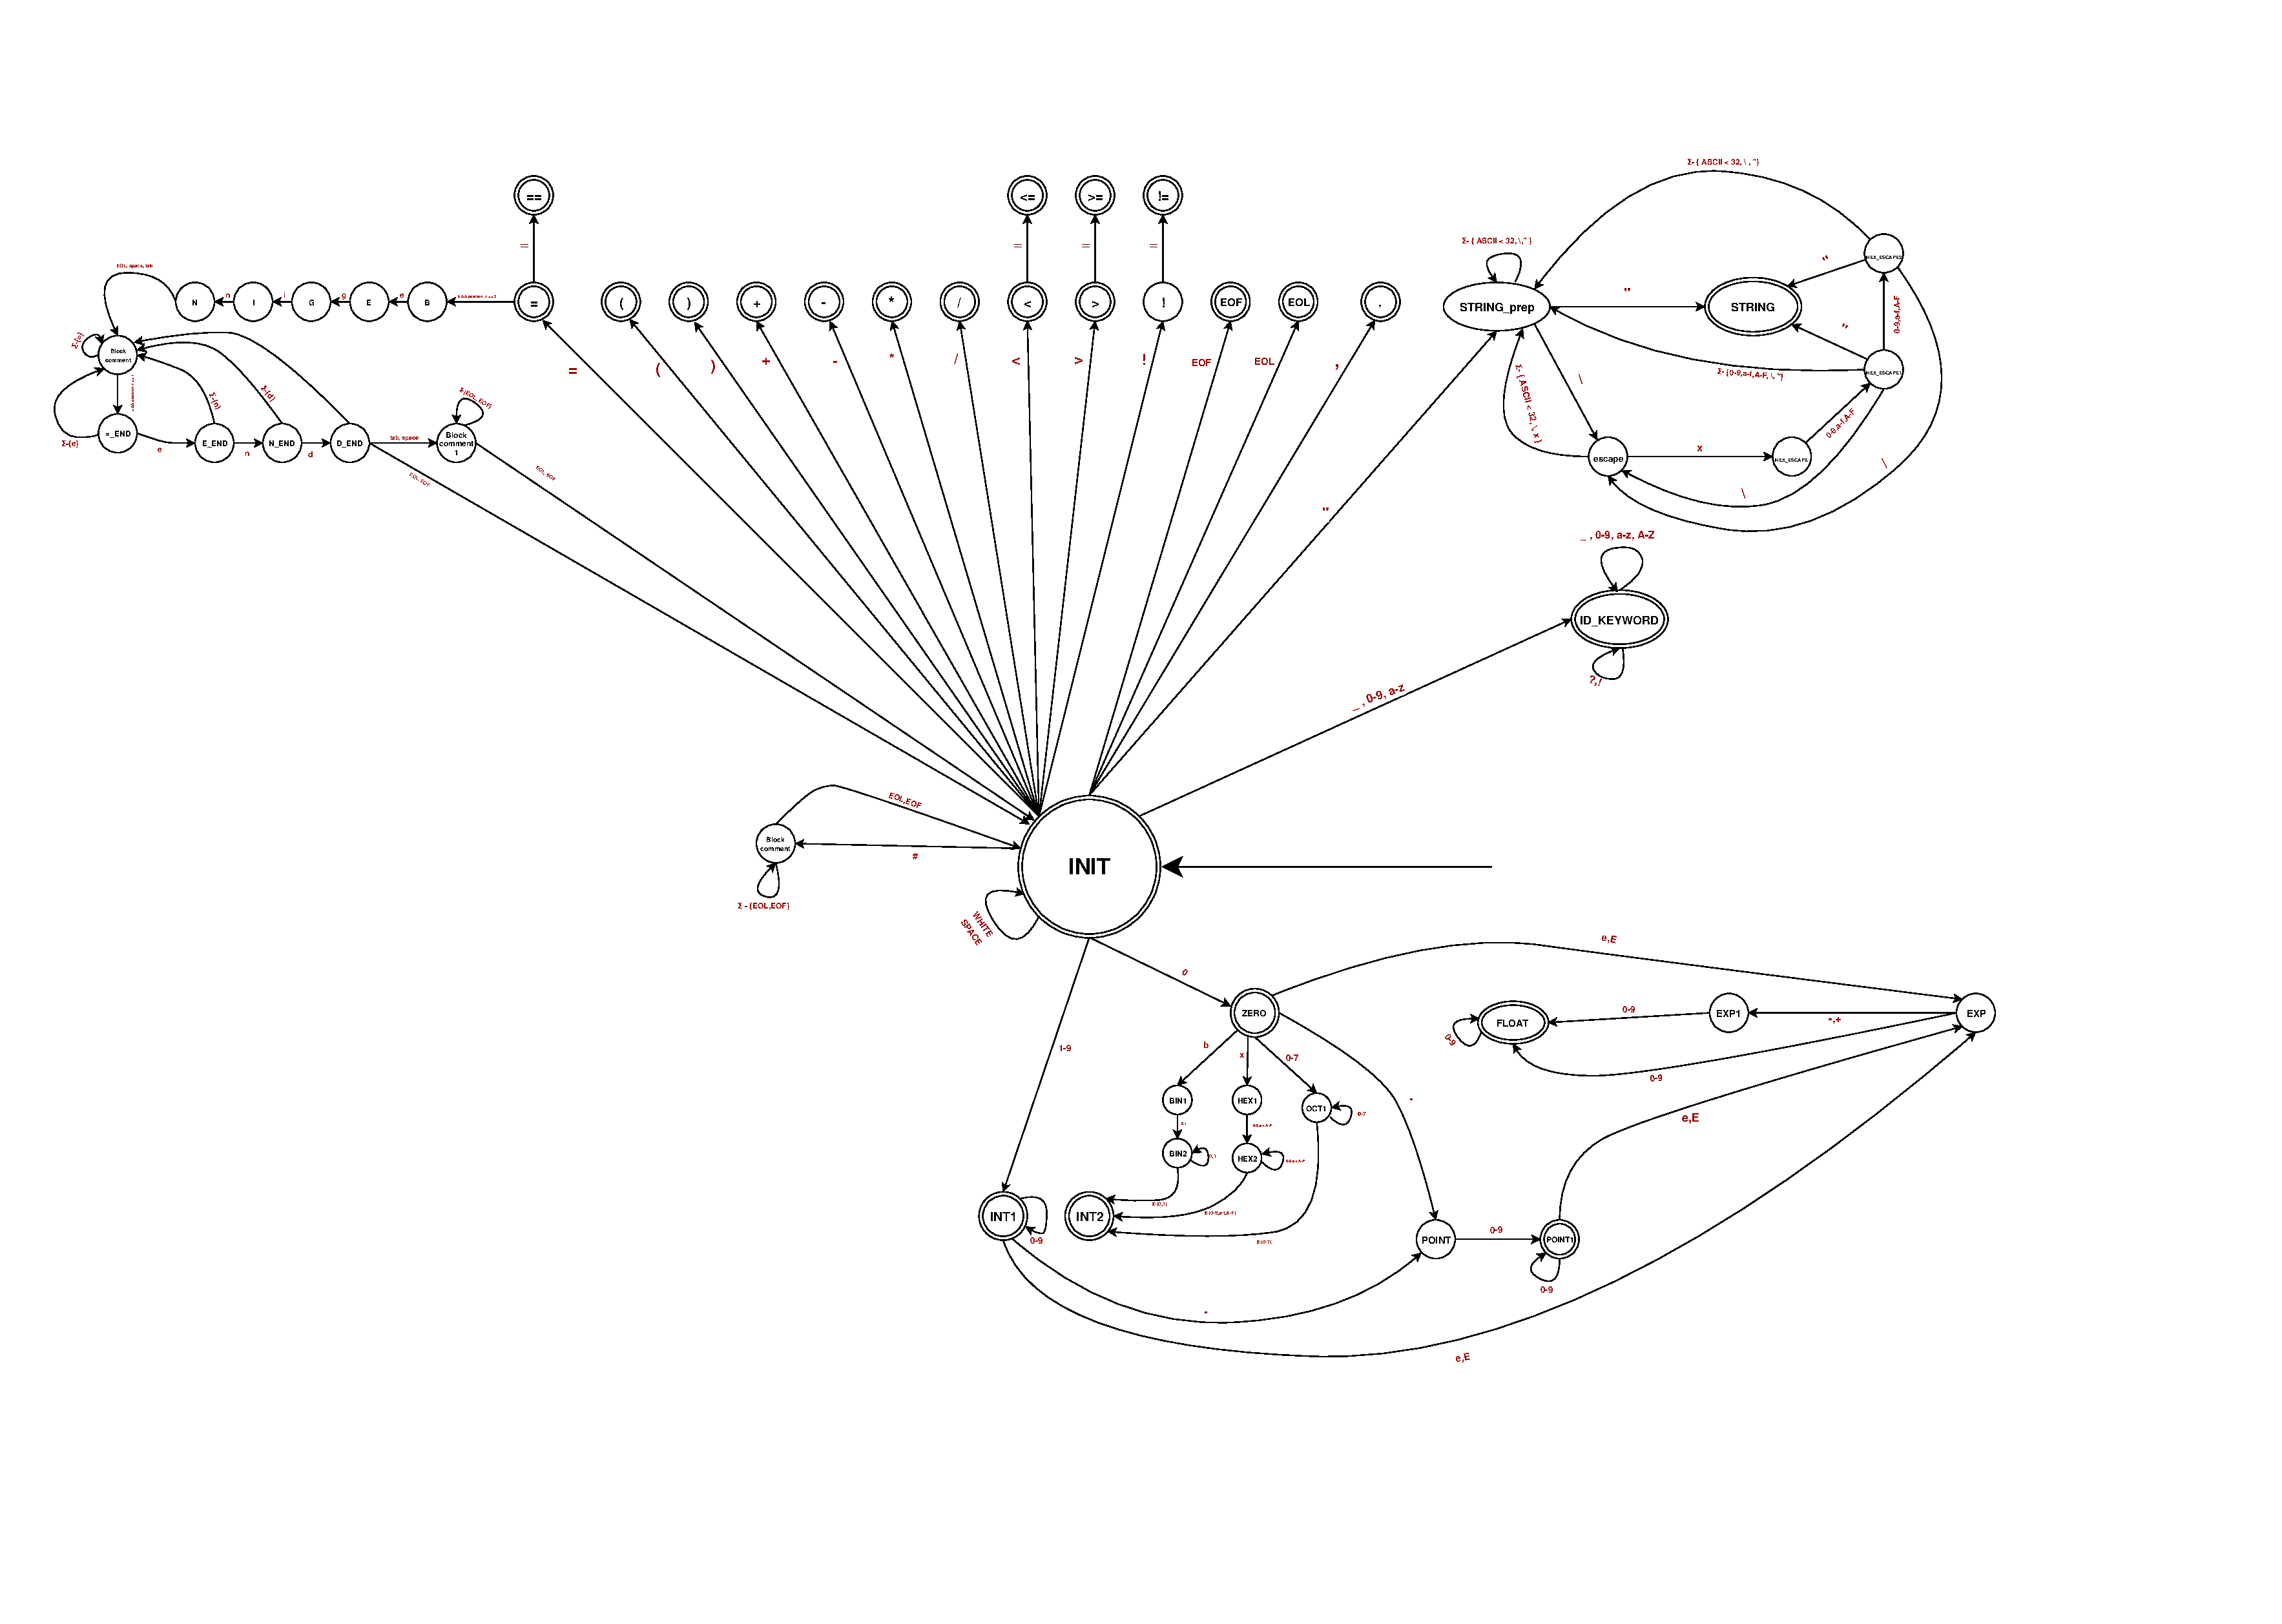
\includegraphics[scale=0.5, center]{konecny_automat.eps}
\end{figure}
\end{landscape}
\end{document}